\documentclass[main.tex]{subfiles}

\begin{document}

% \textcolor{red}{Вводная лекция}

\section{Лекция 18.05.2021 (Байкин А.Н.)}

\subsection{Модели инициации трещины гидроразрыва}

\subsubsection{Моделирование гидроразрыва}

\includegraphics[width=\textwidth, page=111]{HF_slides_2022.pdf}

С точки зрения моделирования гидроразрыва мы с вами по большей части рассматривали распространение уже так называемой развитой трещины, т.е. когда она инициировалась, вышла на направление перпендикулярное минимальным главным напряжениям в пласте и распространяется по определённому закону.

Практика показывает, что эта магистральная трещина распространяется преимущественно в некоторой выделенной плоскости (по крайней мере в однородном пласте).

СЕГОДНЯ мы с вами рассмотрим процесс, который изображён на первом рисунке на слайде, т.е. процесс инициации: есть открытый ствол или перфорация и начинаем закачивать жидкость, растёт давление и спрашивается, при каком давлении порода порвётся и трещина начнёт распространяться.

Есть ещё промежуточный процесс между инициацией трещины и развитой трещиной -- это так называемое начальное распространение трещины: трещина, инициированная из открытого ствола скважины или перфорации (которые могут быть ориентированы под некоторым углом), может быть не перпендикулярна минимальным сжимающим напряжениям, тогда в процессе начального распространения эта трещина попытается выйти в магистральную плоскость каким-то образом.
Во время этого переходного процесса трещина может изгибаться, может перегибаться, что даст дополнительное гидродинамическое сопротивление в этой зоне (вообще говоря можно получить сток); если трещина сильно перегнётся в этой зоне, то это даст неблагоприятные последствия.

\subsubsection{Инициация трещины}

\includegraphics[width=\textwidth, page=112]{HF_slides_2022.pdf}

Здесь представлен небольшой outline нашей сегодняшней беседы.
Будут продемонстрированы результаты группы Чёрного из института вычислительных технологий.

\subsubsection{Расчёт напряжённо-деформированного состояния}

\includegraphics[width=\textwidth, page=113]{HF_slides_2022.pdf}

Сначала давайте поговорим, как формулируется задача об инициации.
Понятно, что у нас есть скважина (с перфорацией) и вокруг есть некоторая упругая среда, представляющая собой породу.
Эта упругая среда подчиняется уравнению равновесия и закону Гука (в самом простом случае без учёта пластичности, нелинейных вкраплений и так далее), также есть связь между деформациями и перемещениями.

Далее необходимо поставить граничные условия.
Здесь на слайде они выписаны в общем виде, но сразу скажу, что это будут граничные условия на бесконечности (или в какой-то дали от ствола скважины -- условной бесконечности; можно показать, что если отойти на расстояние порядка 10 диаметров от ствола скважины, то скважина перестанет влиять на напряжённо-деформированное состояние), а на самой скважине задаётся давление жидкости (которое всегда действует перпендикулярно поверхности, т.е. оно будет действовать по нормали и пытаться как-бы сдвинуть/расширить породу).

Сразу пробегусь, как можно это всё решить численно.
На рисунке на слайде сетка изображена не просто так.
Группа Чёрного предлагает решать эту задачу методом граничных элементов.

\subsubsection{Численные решения уравнений упругого равновесия}

\includegraphics[width=\textwidth, page=114]{HF_slides_2022.pdf}

В прошлом семестре у вас уже был метод граничных элементов.
Он основан на так называемой теореме взаимности.

В чём основная фишка этого метода?
Он позволяет свести вообще говоря трёхмерную задачу к можно сказать двумерной, т.е. когда уравнения и неизвестные записываются в некоторой двумерной поверхности.

Основной минус: матрица системы получается в итоге полностью заполненной -- это является накладными расходами этого метода.

В интегральное соотношение необходимо подставить дискретизацию.
Можно сказать, что это такой метод конечных элементов на поверхности.
И после этого у нас формируется система линейных уравнений.

Это такой в данном случае метод, где можно "<бить пушкой по воробьям"> (в смысле этой задачи по инициации).
Можно задать перфорацию произвольной формы, можно добавить обсадную колонну; здесь же разные варианты могут быть: открытый ствол (когда у нас просто есть скважина, в которую начали качать жидкость -- как порвалась порода, так и порвалась), второй вариант -- взять обсадную колонну и проделать в ней перфорацию (тогда на итог будет влиять и обсадная колонна, и перфорация), третий вариант -- зона перфорирования изолируется так называемым пакером (тогда есть давление после пакера и давление перед пакером).
Т.е. задачи разные, но все они похожие и в принципе каждую из них можно решать (в частности с помощью метода граничных элементов).

Мы пошли по другому пути: студент второго курса нашей программы уехал на 1.5 года во Францию и занимается задачами инициации, но с точки зрения конечных элементов.

Рассказал вам общую информацию про численный метод; давайте пойдём дальше.

\subsubsection{Приближённые решения (2D)}

\includegraphics[width=\textwidth, page=115]{HF_slides_2022.pdf}

Чтобы вы понимали (хотя бы на пальцах), как в простых ситуациях это всё (НДС вблизи скважины) работает, мы сейчас рассмотрим с вами аналитические решения.

С одной стороны, чтобы сформировать некоторое понимание, а с другой стороны, чтобы уже получить какие-то конечные формулы, мы рассмотрим вспомогательную задачу, а именно задачу Кирша.
Это двумерная задача в условиях плоской деформации пластины.
В центре пластины есть отверстие радиуса $a$, которое изначально не нагружено.
Мы начинаем тянуть (растягивать) пластину справа и слева по горизонтали с напряжением $\sigma$, а сверху и снизу напряжений не прикладываем.

Тогда можно показать, что решение задачи (напряжение на границе отверстия) задаётся в следующем виде:
\beq
\sigma_{\theta\theta}(r=a)=\sigma-2\sigma\cos{\!(2\theta)}
\eeq

В книге Тимошенко, Гудиер это получено с помощью функции напряжений.
Видим, что есть зависимость $\sigma_{\theta\theta}$ от угла $\theta$.
Максимальное напряжение на границе отверстия достигается при $\theta=\pm\pi/2$ и равно $3\sigma$.

Давайте усложним задачу, а именно дополнительно приложим растягивающие напряжения $\sigma_y^\infty$ сверху и снизу по вертикали; напряжения $\sigma_x^\infty$ по горизонтали оставим неизменными.
В силу линейности рассматриваемых уравнений упругости решение задачи (напряжение на границе отверстия) в этом случае запишется в следующем виде:
\begin{multline}
\sigma_{\theta\theta}(r=a)=\sigma_x^\infty-2\sigma_x^\infty\cos{\!(2\theta)}+\sigma_y^\infty-2\sigma_y^\infty\cos{\!(2\theta-\pi)}=\\=\left(\sigma_x^\infty+\sigma_y^\infty\right)-2\left(\sigma_x^\infty-\sigma_y^\infty\right)\cos{\!(2\theta)}
\end{multline}

Далее снимем растягивающие напряжения (нулевые напряжения на бесконечности), но начнём в скважину закачивать жидкость с давлением $p_w$.
Тогда получим
\beq\label{sigma_and_p_w}
\sigma_{\theta\theta}=\frac{a^2}{r^2}p_w
\eeq

При $r=a$ напряжение $\sigma_{\theta\theta}=p_w$.
Это означает, что когда вы действуете давлением, то с одной стороны у вас возникает напряжение $\sigma_{rr}=-p_w$, перпендикулярное границе отверстия, а с другой стороны дополнительно появляется окружное напряжение $\sigma_{\theta\theta}=p_w$.
И именно за счёт этого окружного напряжения порода будет рваться.

Используя линейность рассматриваемых уравнений упругости, по принципу суперпозиции можем получить решение комбинированной задачи, когда в главных осях заданы напряжения на бесконечности и задано давление жидкости в скважине.
Получаем:
\begin{multline}\label{Kirsh_itog}
\sigma_{\theta\theta}(r=a)=\sigma_x^\infty-2\sigma_x^\infty\cos{\!(2\theta)}+\sigma_y^\infty-2\sigma_y^\infty\cos{\!(2\theta-\pi)}+p_w=\\=\left(\sigma_x^\infty+\sigma_y^\infty\right)-2\left(\sigma_x^\infty-\sigma_y^\infty\right)\cos{\!(2\theta)}+p_w
\end{multline}

Вам я предлагаю вывести формулу \eqref{sigma_and_p_w} самостоятельно.
Небольшое указание: если будете искать решение в виде $u_r=u_r(r)$, то быстро придёте к результату.

\includegraphics[width=\textwidth, page=116]{HF_slides_2022.pdf}

Посмотрим на решение, которое только что мы с вами получили.

Так как в породе действуют сжимающие напряжения, то мы поменяем знак напряжений на бесконечности $\sigma_x^\infty=-\sigma_{min}$ и $\sigma_y^\infty=-\sigma_{max}$ и подставим их в формулу \eqref{Kirsh_itog}:
\beq
\sigma_{\theta\theta}(r=a)=p_w-\left(\sigma_{max}+\sigma_{min}\right)-2\left(\sigma_{max}-\sigma_{min}\right)\cos{\!(2\theta)}
\eeq

Теперь наша задача понять, в каком месте инициируется трещина.

Самой простой критерий звучит так: как только в какой-то точке скважины растягивающее напряжение достигает некоторого критического значения $\sigma_{\!t}$, тогда возникает разрушение.

Соответственно необходимо решить задачу максимизации функции $\sigma_{\theta\theta}$.
Для этого (ясное дело) можно посчитать производную.
Но в нашем случае всё просто: максимум достигается при $\cos{\!(2\theta)}=-1$, т.е. разрушение будет возникать при $\theta=\pm\pi/2$.

Это соответствует нашим ожиданиям (представлениям о процессе), потому что трещина действительно пойдёт перпендикулярно минимальным сжимающим напряжениям.

Давление инициации:
\beq
p_w=3\sigma_{min}-\sigma_{max}+\sigma_t
\eeq
Здесь стоит заметить, что часто $\sigma_{\!t}$ пренебрегают (говорят, что она мала по сравнению с $\sigma_{min}$ и $\sigma_{max}$ -- напряжение $\sigma_{\!t}$ порядка каких-то мегапаскалей, а напряжения $\sigma_{min}$ и $\sigma_{max}$ порядка нескольких десятков мегапаскалей).

\subsubsection{Приближённые решения (3D)}

\includegraphics[width=\textwidth, page=117]{HF_slides_2022.pdf}

Дальше будем усложнять задачу: во-первых, скважина может быть наклонена и тогда мы не будем находиться в главных осях (в тензоре напряжений могут возникнуть внедиагональные элементы); во-вторых, действуют напряжения $\sigma_{zz}^\infty$ сверху.

\includegraphics[width=\textwidth, page=118]{HF_slides_2022.pdf}

Давайте рассмотрим конкретный пример, как эти формулы уже можно применить.
Представьте, что у вас есть вертикальная скважина: по вертикали действует напряжение $\sigma_3=-10000\text{ psi}$, минимальное горизонтальное напряжение $\sigma_1=-5000\text{ psi}$, максимальное горизонтальное напряжение $\sigma_2=-6500\text{ psi}$.
\\

Упражнение: посчитать давление инициации и угол для горизонтальной скважины.
Здесь есть два варианта: скважина расположена вдоль первого направления (минимальных горизонтальных напряжений) или вдоль второго направления (максимальных горизонтальных напряжений).

\subsubsection{НДС для перфорированной скважины}

\includegraphics[width=\textwidth, page=119]{HF_slides_2022.pdf}

Дальше будем усложнять задачу, а именно добавим перфорацию.

\subsubsection{Примеры для перфорированной скважины}

\includegraphics[width=\textwidth, page=120]{HF_slides_2022.pdf}

\subsubsection{Дополнительные эффекты}

\includegraphics[width=\textwidth, page=121]{HF_slides_2022.pdf}

Что ещё может влиять на инициацию трещины?

Во-первых, это поровое давление, т.е. когда мы начинаем качать жидкость в открытый ствол, то часть жидкости начинает фильтроваться в породу (динамическое воздействие).
Вообще говоря, у нас даже изначально есть некоторый уровень порового давления и это давление уменьшает давление инициации трещины.
По сути оно помогает инициировать трещину.

Во-вторых, температура.

В-третьих, обсадная колонна.

\includegraphics[width=\textwidth, page=122]{HF_slides_2022.pdf}

\subsubsection{Серийные численные расчёты}

\includegraphics[width=\textwidth, page=123]{HF_slides_2022.pdf}

\includegraphics[width=\textwidth, page=124]{HF_slides_2022.pdf}

\includegraphics[width=\textwidth, page=125]{HF_slides_2022.pdf}

\includegraphics[width=\textwidth, page=126]{HF_slides_2022.pdf}

\subsubsection{Критерии инициации трещины}

\includegraphics[width=\textwidth, page=127]{HF_slides_2022.pdf}

\includegraphics[width=\textwidth, page=128]{HF_slides_2022.pdf}

\subsubsection{Учёт эффекта размера}

\includegraphics[width=\textwidth, page=129]{HF_slides_2022.pdf}

\includegraphics[width=\textwidth, page=130]{HF_slides_2022.pdf}

\includegraphics[width=\textwidth, page=131]{HF_slides_2022.pdf}

\includegraphics[width=\textwidth, page=132]{HF_slides_2022.pdf}

\end{document}